\documentclass[12pt, a4paper]{article}

% --- PACKAGES DE BASE ---
\usepackage[utf8]{inputenc}    % Encodage des caractères
\usepackage[T1]{fontenc}       % Encodage de la police
\usepackage[french]{babel}     % Support du français
\usepackage{geometry}          % Gestion des marges
\geometry{hmargin=2.5cm, vmargin=3cm}

% --- MATHÉMATIQUES ---
\usepackage{amsmath, amsfonts, amssymb, amsthm} % Packages mathématiques standards
\usepackage{bm}                % Pour les caractères mathématiques en gras

% --- IMAGES ET COULEURS ---
\usepackage{graphicx}          % Pour inclure des images
\usepackage[dvipsnames]{xcolor} % Pour les couleurs
\usepackage{caption}           % Pour personnaliser les légendes
\usepackage{subcaption}        % Pour les sous-figures
\usepackage{tikz}

% --- CODE (Python) ---
\usepackage{listings}          % Pour insérer votre code source
\lstset{
    language=Python,
    basicstyle=\ttfamily\small,
    keywordstyle=\color{blue},
    stringstyle=\color{OliveGreen},
    commentstyle=\color{gray},
    numbers=left,
    numberstyle=\tiny\color{gray},
    breaklines=true,
    frame=single,
    rulecolor=\color{black}
}

% --- LIENS HYPERTEXTES (à charger en dernier) ---
\usepackage[hidelinks]{hyperref}

% --- MACROS PERSONNALISÉES ---
\newcommand{\E}{\mathbb{E}}    % Espérance
\newcommand{\Prob}{\mathbb{P}} % Probabilité
\newcommand{\R}{\mathbb{R}}    % Réels
\newcommand{\norm}[1]{\left\lVert#1\right\rVert}

% --- INFORMATIONS DU RAPPORT ---
\title{Projet de Processus Stochastiques \\ \Large Détection de motifs par méthodes MCMC}
\author{Franck Duval HEUBA - S227629}
\date{Année Académique 2025-2026}

\begin{document}

\maketitle

\tableofcontents
\newpage

% ---------------------------------------------------------
% PREMIÈRE PARTIE
% ---------------------------------------------------------
\section{Chaînes de Markov et échantillonnage de Gibbs}

\subsection{Chaînes de Markov}

\subsubsection{Estimation de la matrice P}

Pour modéliser la séquence d'ADN fournie (\texttt{seq1}) sous forme de chaîne de Markov, 
nous devons estimer sa matrice de transition $P$. Les états de la chaîne correspondent aux 
quatre nucléotides, numérotés de 1 à 4 : A (1), C (2), G (3), et T (4).

La probabilité de transition de l'état $i$ vers l'état $j$, notée $P_{i,j}$, 
s'estime par la méthode du maximum de vraisemblance (MLE). 
Cet estimateur correspond à la fréquence empirique des transitions 
observées dans la séquence :

\begin{equation}
    \hat{P}_{i,j} = \frac{N_{i,j}}{\sum_{k=1}^{4} N_{i,k}}
\end{equation}
où $N_{i,j}$ représente le nombre de fois où le nucléotide $i$ est immédiatement 
suivi du nucléotide $j$ dans \texttt{seq1}.

En appliquant cette formule sur notre séquence, nous obtenons la 
matrice de transition empirique suivante (arrondie à 3 décimales) :

\begin{equation}
    P = 
    \begin{pmatrix}
        P_{AA} & P_{AC} & P_{AG} & P_{AT} \\
        P_{CA} & P_{CC} & P_{CG} & P_{CT} \\
        P_{GA} & P_{GC} & P_{GG} & P_{GT} \\
        P_{TA} & P_{TC} & P_{TG} & P_{TT}
    \end{pmatrix}
    =
    \begin{pmatrix}
        0.097 & 0.505 & 0.278 & 0.120 \\ % Row A
        0.253 & 0.246 & 0.262 & 0.239 \\ % Row C
        0.311 & 0.493 & 0.108 & 0.089 \\ % Row G
        0.696 & 0.098 & 0.098 & 0.108    % Row T
    \end{pmatrix}
\end{equation}

\subparagraph{Diagramme d'états}
Le graphe orienté ci-dessous illustre la dynamique de cette chaîne de Markov. 
Les nœuds représentent les états (A, C, G, T) et les arêtes indiquent les probabilités 
de transition $\hat{P}_{i,j}$.

\begin{figure}[ht]
    \centering
    \begin{tikzpicture}[->, >=stealth, node distance=4cm, auto, thick, state/.style={circle, draw, minimum size=1.5cm, fill=blue!5}]
        % Nœuds
        \node[state] (A) {A (1)};
        \node[state, right of=A] (C) {C (2)};
        \node[state, below of=A] (T) {T (4)};
        \node[state, right of=T] (G) {G (3)};

        % Transitions depuis A (Row 1)
        \path (A) edge[loop above] node {0.097} (A)
              (A) edge[bend left] node {0.505} (C)
              (A) edge[bend left=15] node[near start] {0.278} (G)
              (A) edge[bend left] node {0.120} (T);

        % Transitions depuis C (Row 2)
        \path (C) edge[loop above] node {0.246} (C)
              (C) edge[bend left] node {0.253} (A)
              (C) edge[bend left] node {0.239} (T)
              (C) edge[bend left=15] node[near start] {0.262} (G);

        % Transitions depuis G (Row 3)
        \path (G) edge[loop below] node {0.108} (G)
              (G) edge[bend left] node {0.493} (C)
              (G) edge[bend left=15] node[near start] {0.311} (A)
              (G) edge[bend left] node {0.089} (T);

        % Transitions depuis T (Row 4)
        \path (T) edge[loop below] node {0.108} (T)
              (T) edge[bend left] node {0.696} (A)
              (T) edge[bend left=15] node[near start] {0.098} (C)
              (T) edge[bend left] node {0.098} (G);
    \end{tikzpicture}
    \caption{Diagramme d'états de la chaîne de Markov modélisant \texttt{seq1}.}
    \label{fig:markov_seq1}
\end{figure}

\subsubsection{Évolution temporelle}

Pour étudier la dynamique temporelle de notre chaîne de Markov, nous calculons la distribution de probabilité des états au temps $t$, notée $u_t$. Si la chaîne possède un vecteur de probabilité initial $u_0$, la distribution au temps $t$ est donnée par l'équation :
\begin{equation}
    u_t = u_0 P^t
\end{equation}

Nous avons simulé cette évolution sur 20 étapes temporelles pour deux conditions initiales distinctes :
\begin{enumerate}
    \item Une distribution initiale uniforme : $u_0 = (0.25, 0.25, 0.25, 0.25)$.
    \item Un départ certain depuis le nucléotide 'C' : $u_0 = (0, 1, 0, 0)$.
\end{enumerate}

La Figure \ref{fig:evolution_markov} illustre les résultats obtenus.

\begin{figure}[ht]
    \centering
    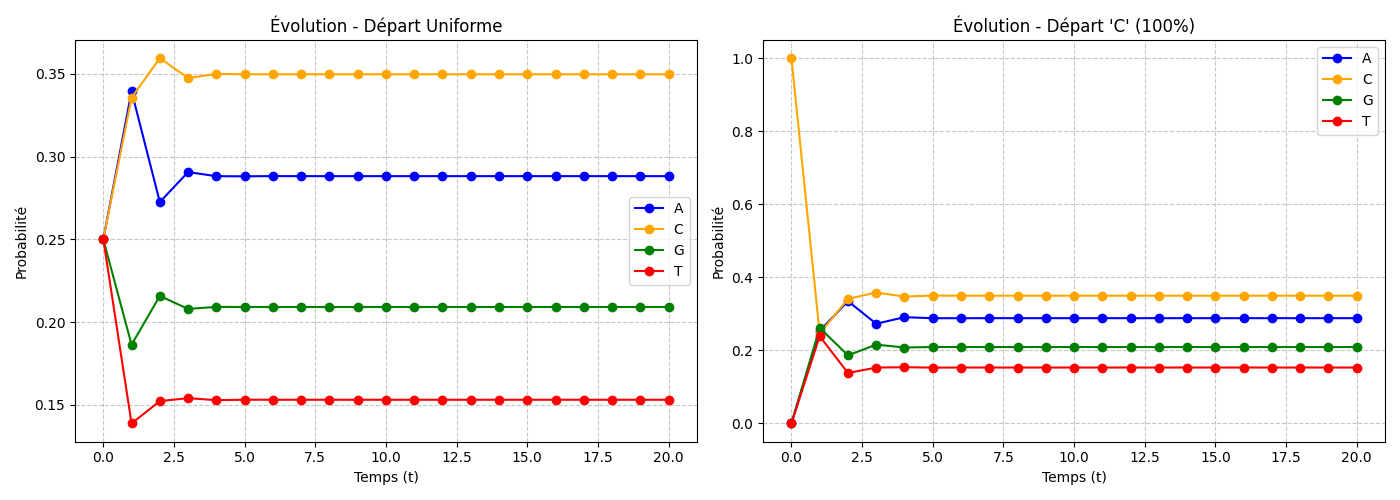
\includegraphics[width=1\textwidth]{images/evolution_markov.png}
    \caption{Évolution de la probabilité de se trouver dans chaque état (A, C, G, T) au cours du temps, pour deux conditions initiales différentes.}
    \label{fig:evolution_markov}
\end{figure}

\subparagraph{Analyse des observations}
Nous remarquons que, bien que les trajectoires des premières étapes 
soient très différentes selon la condition initiale, les probabilités 
finissent par se stabiliser et converger vers des valeurs constantes après 
environ $t = 3$ itérations. 

Indépendamment de la condition initiale, les probabilités convergent toutes vers le même ordre
$P(C) > P(A) > P(G) > P(T)$. Les différences observées lors des premières étapes (phase transitoire) 
disparaissent rapidement, démontrant que la chaîne « oublie » son point de départ en convergeant 
vers sa distribution stationnaire unique.

En calculant la matrice $P^t$ pour une valeur de $t$ suffisamment grande (par exemple $t=50$), nous observons le résultat suivant :
\begin{equation}
P^{50} \approx
    \begin{pmatrix}
        0.2881 & 0.3497 & 0.2091 & 0.1531 \\
        0.2881 & 0.3497 & 0.2091 & 0.1531 \\
        0.2881 & 0.3497 & 0.2091 & 0.1531 \\
        0.2881 & 0.3497 & 0.2091 & 0.1531
    \end{pmatrix}
\end{equation}

Les lignes de la matrice $P^t$ deviennent toutes identiques. 
Cela s'explique mathématiquement : l'élément $(i,j)$ de $P^t$ représente la probabilité 
de se trouver dans l'état $j$ après $t$ étapes en partant de l'état $i$. Le fait que toutes 
les lignes soient égales signifie que pour un temps $t$ suffisamment long, la probabilité 
d'être dans un état donné ne dépend plus du tout de l'état de départ. La chaine a "oublié" 
sa condition initiale lors qu'elle converge vers la distribution stationnaire.

\subsubsection{Distribution stationnaire}

La distribution stationnaire d'une chaîne de Markov, 
notée $\pi_\infty$, est une distribution de probabilité qui 
reste invariante lors de l'application de la matrice de transition $P$. 
Mathématiquement, elle satisfait le système d'équations suivant :
\begin{equation}
    \pi_\infty P = \pi_\infty \quad \text{soumis à la contrainte} \quad \sum_{i \in \mathcal{S}} (\pi_\infty)_i = 1
\end{equation}

D'un point de vue algébrique, cela signifie que $\pi_\infty$ est le vecteur 
propre à gauche de la matrice $P$ associé à la valeur propre $\lambda = 1$.

Plutôt que d'estimer cette distribution en élevant $P$ à une grande puissance 
(comme fait précédemment), nous l'avons calculée analytiquement en procédant 
à la décomposition spectrale de la transposée de la matrice $P$ ($P^T$).

Après extraction du vecteur propre correspondant à la valeur 
propre $\lambda = 1$ et normalisation pour que la somme de ses éléments vaille 1, 
nous obtenons la distribution stationnaire suivante :
\begin{equation}
    \pi_\infty = 
    \begin{pmatrix}
        \pi_A \\ \pi_C \\ \pi_G \\ \pi_T
    \end{pmatrix}^T
    = 
    \begin{pmatrix}
        0.2881 \\ 0.3497 \\ 0.2091 \\ 0.1531 
    \end{pmatrix}^T
\end{equation}

\subparagraph{Conclusion sur la convergence}
Nous constatons que ce calcul analytique direct corrobore parfaitement 
l'observation empirique de la question précédente (1.1.2). Les valeurs de $\pi_\infty$ 
correspondent exactement aux probabilités vers lesquelles les lignes de la matrice $P^{50}$ 
avaient convergé. La chaîne de Markov modélisant notre séquence d'ADN possède donc 
bien une unique distribution stationnaire vers laquelle le système tend asymptotiquement, 
quelle que soit sa condition initiale.

\subsubsection{Ergodicité}

Une chaîne de Markov est dite ergodique si elle est irréductible 
(il est possible d'atteindre n'importe quel état depuis n'importe quel autre) et apériodique. 
Pour une telle chaîne, le théorème ergodique stipule que la proportion du temps passé dans un 
état $i$ sur une trajectoire infiniment longue converge vers la probabilité 
stationnaire $\pi_i$ de cet état :
\begin{equation}
    \lim_{N \to \infty} \frac{1}{N} \sum_{t=1}^N \mathbf{1}_{\{X_t = i\}} = \pi_i
\end{equation}

Pour vérifier expérimentalement cette propriété, nous avons simulé une trajectoire de la 
chaîne en générant une nouvelle séquence artificielle de $N = 50\,000$ nucléotides. À 
chaque étape, la transition vers le nucléotide suivant a été tirée aléatoirement en respectant 
strictement les probabilités de la matrice de transition $P$ estimée à la Question 1.1.1. 
Nous avons ensuite calculé les fréquences empiriques d'apparition de chaque nucléotide dans 
cette séquence générée.

Le tableau ci-dessous compare ces fréquences empiriques temporelles avec la distribution 
stationnaire $\pi_\infty$ calculée analytiquement à la Question 1.1.3 :

\begin{center}
\renewcommand{\arraystretch}{1.2} % Donne un peu d'espace dans les lignes du tableau
\begin{tabular}{|c|c|c|}
    \hline
    \textbf{Nucléotide} & \textbf{Fréquence empirique (N=50 000)} & \textbf{Distribution stationnaire ($\pi_\infty$)} \\
    \hline
    A & 0.2879 & 0.2881 \\ 
    C & 0.3483 & 0.3497 \\ 
    G & 0.2117 & 0.2091 \\ 
    T & 0.1521 & 0.1531 \\ 
    \hline
\end{tabular}
\end{center}

\subparagraph{Conclusion}
Nous constatons que les fréquences empiriques observées sur une longue réalisation de la 
chaîne sont extrêmement proches des probabilités de la distribution stationnaire $\pi_\infty$ 
(aux fluctuations statistiques d'échantillonnage près). Cela confirme numériquement que 
notre modèle de séquence d'ADN forme bien une chaîne de Markov ergodique : 
l'exploration temporelle du système (simulée sur 50 000 étapes) reflète fidèlement son 
équilibre spatial théorique.

\subsubsection{Évaluation de séquences}

\paragraph{ }
\subparagraph{Comparaison des fréquences empiriques}
Avant d'évaluer les séquences avec notre modèle de Markov, 
nous avons calculé la fréquence d'apparition simple (modèle d'ordre 0) de chaque 
nucléotide pour les trois séquences fournies :

\begin{center}
\renewcommand{\arraystretch}{1.2}
\begin{tabular}{|l|c|c|c|c|}
    \hline
    \textbf{Séquence} & \textbf{Fréq. A} & \textbf{Fréq. C} & \textbf{Fréq. G} & \textbf{Fréq. T} \\
    \hline
    Séquence 1 & 0.2885 & 0.3495 & 0.2090 & 0.1530 \\ 
    Séquence 2 & 0.3060 & 0.3415 & 0.1970 & 0.1555 \\ 
    Séquence 3 & 0.2845 & 0.3605 & 0.1985 & 0.1565 \\ 
    \hline
\end{tabular}
\end{center}

L'analyse de ce tableau révèle que:  
\textit{Seq1, Seq2 et Seq3 ont des distributions très similaires.}

\subparagraph{Évaluation par le modèle de Markov}
Afin d'évaluer plus finement dans quelle mesure ces séquences sont compatibles avec 
la dynamique de \texttt{seq1}, nous calculons la probabilité d'observer chacune d'entre 
elles sous l'hypothèse qu'elles ont été générées par notre chaîne de Markov.

La vraisemblance d'une séquence $S = (x_1, x_2, \dots, x_L)$ s'écrit :
\begin{equation}
    \Prob(S \mid P) = \pi_\infty(x_1) \prod_{t=1}^{L-1} P_{x_t, x_{t+1}}
\end{equation}

Pour éviter l'underflow numérique dû au produit de milliers de probabilités, 
nous utilisons la log-vraisemblance moyenne par nucléotide :
\begin{equation}
    \frac{1}{L} \log \Prob(S \mid P) = \frac{1}{L} \left( \log(\pi_\infty(x_1)) + \sum_{t=1}^{L-1} \log(P_{x_t, x_{t+1}}) \right)
\end{equation}

Les résultats obtenus pour les trois séquences sont les suivants :
\begin{itemize}
    \item \textbf{Séquence 1} : Log-vraisemblance moyenne = -1.2140
    \item \textbf{Séquence 2} : Log-vraisemblance moyenne = -1.4864
    \item \textbf{Séquence 3} : Log-vraisemblance moyenne = -1.2005
\end{itemize}

\subparagraph{Conclusion : Comparaison et puissance du modèle de Markov}

L'analyse conjointe des fréquences empiriques et des log-vraisemblances 
révèle l'intérêt fondamental de la modélisation par chaînes de Markov. 

Dans un premier temps, l'observation des fréquences d'apparition simples 
montre que les trois séquences possèdent une composition globale quasi-identique 
(environ 29\% de A, 35\% de C, 20\% de G et 16\% de T). Sur la seule 
base de ces comptages, on pourrait conclure que ces trois séquences proviennent 
du même processus stochastique.

Cependant, l'évaluation par la log-vraisemblance met en lumière une réalité différente, 
car elle prend en compte la dynamique temporelle (les probabilités de transition entre 
nucléotides adjacents) :
\begin{itemize}
    \item \textbf{La Séquence 3} obtient une log-vraisemblance moyenne ($-1.2005$) extrêmement proche de celle de la Séquence 1 ($-1.2140$), sur laquelle le modèle a été entraîné. Cela prouve que la Séquence 3 partage la même "signature" de transitions stochastiques que la Séquence 1. Elles ont très certainement été générées par le même processus.
    \item \textbf{La Séquence 2}, en revanche, obtient une log-vraisemblance nettement inférieure ($-1.4864$). L'échelle étant logarithmique sur 2000 caractères, cette différence indique que la probabilité que la Séquence 2 ait été générée par notre matrice $P$ est infime. 
\end{itemize}

Nous pouvons donc conclure que bien que la Séquence 2 utilise les mêmes proportions de 
nucléotides que la Séquence 1, leur ordonnancement est fondamentalement différent. 
Le modèle de Markov réussit là où le simple comptage échoue : il détecte que la 
Séquence 2 est une anomalie générée par un processus 
(ou un modèle de fond biologique) distinct.


\newpage
\subsection{Échantillonnage de Gibbs}

\subsubsection{Preuve de la stationnarité de l'échantillonneur de Gibbs}

L'objectif est de démontrer que la distribution jointe $p(Y)$ est la distribution 
stationnaire de la chaîne de Markov construite par l'algorithme de Gibbs. 
Pour ce faire, nous allons prouver que cette chaîne satisfait la 
\textbf{condition de balance détaillée}.

\subparagraph{Définition du noyau de transition}
Soit $y = (y_1, \dots, y_n)$ l'état actuel de la chaîne. Dans l'échantillonneur de 
Gibbs à balayage aléatoire, une transition vers un état $y'$ se déroule comme suit :
\begin{enumerate}
    \item On choisit un indice $j \in \{1, \dots, n\}$ avec une probabilité uniforme $1/n$.
    \item On met à jour la $j$-ème composante en tirant $y'_j \sim p(Y_j \mid Y_{-j} = y_{-j})$.
\end{enumerate}
L'état d'arrivée est donc $y' = (y'_j, y_{-j})$. Si $y$ et $y'$ diffèrent 
par plus d'une composante, la probabilité de transition $P(y \to y')$ est nulle.

\subparagraph{Démonstration par la balance détaillée}
Considérons deux états $y$ et $y'$ ne différant que par la composante $j$. 
La probabilité de transition est :
\begin{equation}
    P(y \to y') = \frac{1}{n} p(y'_j \mid y_{-j})
\end{equation}
Vérifions si le flux de probabilité entre $y$ et $y'$ est équilibré, 
c'est-à-dire si $p(y)P(y \to y') = p(y')P(y' \to y)$.

En utilisant la définition de la probabilité conditionnelle 
$p(y) = p(y_j \mid y_{-j}) p(y_{-j})$, le membre de gauche devient :
\begin{align}
    p(y) P(y \to y') &= \left[ p(y_j \mid y_{-j}) p(y_{-j}) \right] \times \left[ \frac{1}{n} p(y'_j \mid y_{-j}) \right] \nonumber \\
    &= \frac{1}{n} p(y_j \mid y_{-j}) p(y'_j \mid y_{-j}) p(y_{-j})
\end{align}

De la même manière, pour le flux inverse partant de $y' = (y'_j, y_{-j})$ vers $y = (y_j, y_{-j})$ :
\begin{align}
    p(y') P(y' \to y) &= \left[ p(y'_j \mid y_{-j}) p(y_{-j}) \right] \times \left[ \frac{1}{n} p(y_j \mid y_{-j}) \right] \nonumber \\
    &= \frac{1}{n} p(y'_j \mid y_{-j}) p(y_j \mid y_{-j}) p(y_{-j})
\end{align}

Nous observons que les deux expressions sont identiques. La condition de 
balance détaillée est respectée :
\begin{equation}
    p(y) P(y \to y') = p(y') P(y' \to y)
\end{equation}

\subparagraph{Conclusion}
La balance détaillée implique que la distribution $p(Y)$ est invariante par le noyau 
de transition de Gibbs. Puisque $p(Y)$ est stationnaire et que la chaîne est 
(sous réserve de positivité de la densité) irréductible et apériodique, la chaîne de 
Markov convergera vers $p(Y)$ indépendamment de l'état initial $y^{(0)}$.

\textit{Note sur l'implémentation :} Lors de la mise en œuvre pratique (Question 1.2.2), le tirage selon la loi conditionnelle $p(Y_j \mid Y_{-j})$ sera effectué en appliquant la \textbf{Proposition 3.6.3} via la méthode de la transformée inverse.

\subsubsection{Implémentation et comparaison des stratégies de balayage}

\subparagraph{(a) Choix de la distribution jointe $Q_Y$}
Nous définissons une distribution jointe sur deux variables 
$Y_1, Y_2 \in \{1, 2, 3, 4\}$ par la matrice $Q_Y \in \mathbb{R}^{4 \times 4}$ suivante :
\begin{equation}
    [Q_Y]_{i,j} = \frac{i+j}{80}, \quad \forall i,j \in \{1, \dots, 4\}
\end{equation}
Cette distribution respecte la condition de positivité ($Q_Y > 0$), 
ce qui garantit que la chaîne de Markov est \textbf{irréductible} et \textbf{apériodique}. 
Ces deux conditions assurent, selon la théorie du point 1, que l'algorithme de Gibbs convergera 
vers l'unique distribution stationnaire $Q_Y$.

\subparagraph{(b) Réalisation par balayage aléatoire (Algorithme 1)}
Nous avons généré une chaîne de $50\,000$ itérations en choisissant à chaque étape 
l'indice de la variable à mettre à jour uniformément dans $\{1, 2\}$. Les tirages selon les 
lois conditionnelles $P(Y_1 \mid Y_2)$ et $P(Y_2 \mid Y_1)$ ont été effectués via la méthode 
de la transformée inverse. La Figure \ref{fig:gibbs_comp} montre que les fréquences empiriques 
épousent parfaitement les valeurs théoriques de $Q_Y$.

\subparagraph{(c) Balayage systématique et conclusion}
L'expérience a été répétée en utilisant un balayage systématique 
(mise à jour de $Y_1$ puis de $Y_2$ à chaque itération). Les résultats obtenus 
sont statistiquement identiques à ceux du balayage aléatoire. 

\begin{figure}[ht]
    \centering
    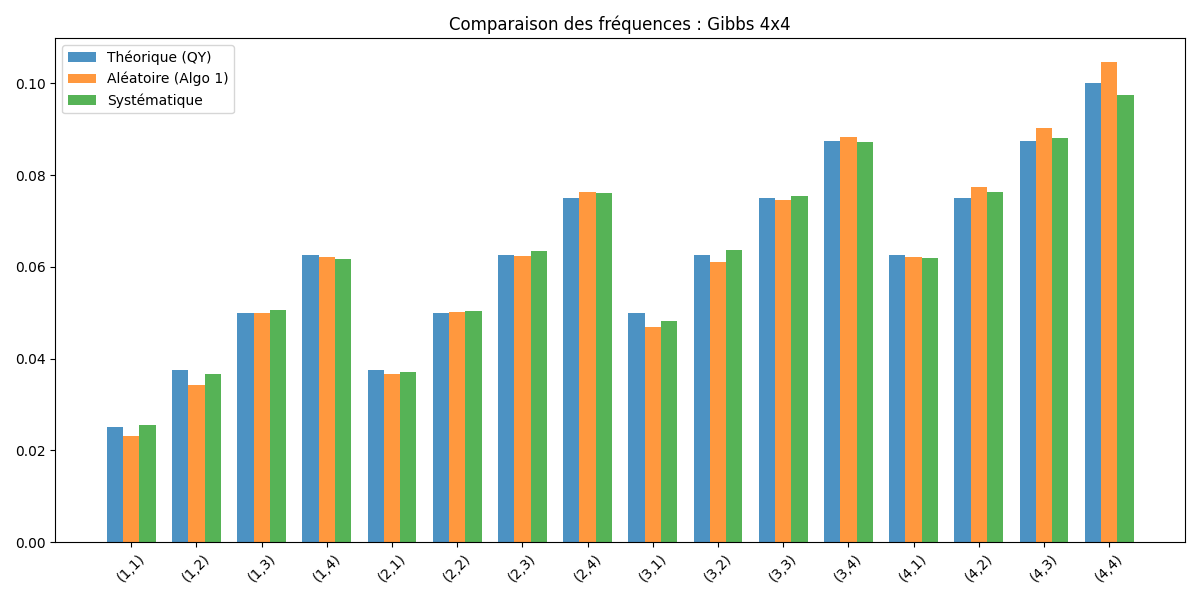
\includegraphics[width=0.9\textwidth]{./images/comparaison_gibbs.png}
    \caption{Comparaison des fréquences d'états pour les deux stratégies de balayage de Gibbs par rapport à la distribution cible.}
    \label{fig:gibbs_comp}
\end{figure}

En conclusion, les deux methodes de balayage (aléatoire et systématique) 
conduisent à des résultats similaires en termes de convergence vers la distribution cible $Q_Y$.

\newpage
\section{Détection de motifs}

\subsection{Dérivations mathématiques}
\paragraph{Question 2.2.1 : Lois conditionnelles de l'échantillonneur de Gibbs}

Dans le cadre de la découverte de motifs \textit{de novo}, l'échantillonneur de Gibbs 
alterne entre l'échantillonnage des paramètres du motif $\Theta$ et l'échantillonnage 
des positions de départ $\mathcal{A} = \{A_1, \dots, A_N\}$. Nous dérivons ci-dessous 
les deux distributions conditionnelles nécessaires à cet algorithme.

\subparagraph{1. Distribution du profil de motif sachant les positions : $p(\Theta \mid \mathcal{A}, \mathcal{S}, \Phi)$}

Par l'application du théorème de Bayes, la distribution a posteriori des paramètres du 
motif est proportionnelle au produit de la vraisemblance des données et de la 
distribution a priori :
\begin{equation}
    p(\Theta \mid \mathcal{A}, \mathcal{S}, \Phi) \propto p(\mathcal{S} \mid \mathcal{A}, \Theta, \Phi) \cdot p(\Theta)
\end{equation}

Pour chaque colonne $j \in \{1, \dots, W\}$ du motif, nous modélisons la 
distribution a priori $p(\Theta_j)$ par une loi de Dirichlet de paramètres 
$\alpha = (\alpha_A, \alpha_C, \alpha_G, \alpha_T)$ :
\begin{equation}
    p(\Theta_j) \sim \text{Dirichlet}(\alpha) \propto \prod_{i \in \{A,C,G,T\}} \Theta_{i,j}^{\alpha_i - 1}
\end{equation}

Étant donné les positions $\mathcal{A}$, les sous-séquences correspondant 
aux motifs sont parfaitement identifiées. Soit $n_{i,j}$ le nombre d'occurrences du 
nucléotide $i$ à la position $j$ du motif à travers toutes les séquences de 
$\mathcal{S}$. La vraisemblance de ces observations suit une loi multinomiale :
\begin{equation}
    p(\text{motifs} \mid \Theta) \propto \prod_{i \in \{A,C,G,T\}} \Theta_{i,j}^{n_{i,j}}
\end{equation}

Puisque la loi de Dirichlet est l'a priori conjugué de la loi multinomiale, 
le produit des deux équations précédentes montre que la distribution a posteriori pour 
chaque colonne $j$ reste une loi de Dirichlet, dont les paramètres sont mis à jour en 
ajoutant les comptages observés $n_{i,j}$ aux pseudo-comptes $\alpha_i$ :
\begin{equation}
    \Theta_j \mid \mathcal{A}, \mathcal{S} \sim \text{Dirichlet}(\alpha_A + n_{A,j}, \alpha_C + n_{C,j}, \alpha_G + n_{G,j}, \alpha_T + n_{T,j})
\end{equation}

\subparagraph{2. Distribution de la position sachant le motif : $p(A_k = a \mid \mathcal{A}_{-k}, \Theta, \mathcal{S}, \Phi)$}

Nous cherchons la probabilité que le motif commence à la position $a$ dans la 
séquence $S_k$, sachant le profil $\Theta$. La position $A_k$ est conditionnellement 
indépendante des autres positions $\mathcal{A}_{-k}$ étant donné $\Theta$.

Par le théorème de Bayes, cette probabilité est proportionnelle à la probabilité de 
générer la séquence $S_k$ avec un motif commençant en $a$ :
\begin{equation}
    P(A_k = a \mid \Theta, S_k, \Phi) = \frac{P(S_k \mid A_k = a, \Theta, \Phi) P(A_k = a)}{\sum_{a'} P(S_k \mid A_k = a', \Theta, \Phi) P(A_k = a')}
\end{equation}

En supposant un a priori uniforme sur les positions possibles ($P(A_k = a)$ constant), nous pouvons évaluer la vraisemblance de la séquence. La séquence est composée de la région du motif (générée par $\Theta$) et du reste de la séquence (généré par le modèle de fond $\Phi$). 

Pour simplifier les calculs, nous divisons cette vraisemblance par la probabilité 
constante $P(S_k \mid \Phi)$ (probabilité que toute la séquence soit du bruit de fond). 
Les termes du bruit de fond s'annulent partout, sauf sur la fenêtre du motif, ce qui 
nous donne le poids $w_a$ :
\begin{equation}
    w_a = \prod_{j=0}^{W-1} \frac{\Theta_{S_{k, a+j}, j}}{\Phi_{S_{k, a+j}}}
\end{equation}
où $S_{k, a+j}$ est le nucléotide présent à la position $a+j$ dans la séquence $S_k$.

La probabilité conditionnelle est finalement obtenue en normalisant ces poids sur 
toutes les positions de départ valides (de $1$ à $L-W+1$, où $L$ est la longueur de la 
séquence) :
\begin{equation}
    P(A_k = a \mid \Theta, S_k, \Phi) = \frac{w_a}{\sum_{a'=1}^{L-W+1} w_{a'}}
\end{equation}
C'est dans cette distribution discrète que la nouvelle position $A_k$ sera 
échantillonnée (par la méthode de la transformée inverse vue à la Partie 1).

\subsection{Implémentation et gestion des décalages}
\paragraph{Question 2.2.2 : Architecture de l'algorithme de Gibbs}

L'algorithme a été implémenté en Python en suivant scrupuleusement les 
dérivations de la question 2.2.1. Les points clés de notre implémentation 
sont les suivants :

\begin{enumerate}
    \item \textbf{Stabilité numérique :} Le calcul des poids $w_a$ pour les positions utilise le ratio entre la probabilité sous le modèle du motif $\Theta$ et le modèle de fond $\Phi$. Cela permet de mettre en évidence le signal du motif par rapport au bruit.
    \item \textbf{Tirage de Dirichlet :} Nous utilisons la fonction \texttt{numpy.random.dirichlet} pour échantillonner la matrice $\Theta$. Les pseudo-comptes $\alpha$ sont fixés à $1$ (prior de Laplace) pour assurer qu'aucun nucléotide n'ait une probabilité nulle, ce qui rendrait le calcul des ratios impossible.
    \item \textbf{Gestion du Phase Shift :} Un problème classique de l'échantillonneur de Gibbs est sa tendance à converger vers un motif décalé de quelques bases (optimum local). Pour pallier cela, nous avons introduit un mouvement de décalage global (Phase Shift) toutes les 10 itérations. Ce mouvement propose de décaler l'ensemble des positions $\mathcal{A}$ d'une unité. Ce saut permet à l'algorithme de s'échapper d'un alignement imparfait.
\end{enumerate}

\subparagraph{Pseudo-code de la boucle principale}
\begin{lstlisting}
Initialiser A au hasard
Pour i de 1 a MaxIter:
    1. Compter les nucleotides dans les fenetres definies par A
    2. Tirer Theta ~ Dirichlet(alpha + counts)
    3. Pour chaque sequence k:
        Recalculer les poids w_a pour chaque position de depart
        Tirer Ak ~ Multinomiale(Normaliser(w))
    4. Si i % 10 == 0: 
        Tenter un Phase Shift (Metropolis-Hastings)
\end{lstlisting}

\subsection{Expérimentations et évaluation (Question 2.2.3)}

Afin d'évaluer quantitativement les performances de notre implémentation de l'échantillonneur de Gibbs, nous avons utilisé deux métriques standards en découverte de motifs :
\begin{itemize}
    \item \textbf{Le Score de Consensus (Contenu en Information) :} Il mesure la conservation du motif trouvé en calculant l'entropie de Shannon sur la matrice $\Theta$. Pour un motif de longueur $W$, le score maximal est de $2W$ bits.
    \item \textbf{L'Average Jaccard Index (AJI) :} Il mesure le taux de chevauchement moyen entre les positions prédites par notre algorithme et les positions réelles connues (fournies dans les fichiers de vérité terrain). Un score de 1.0 indique une prédiction parfaite sur toutes les séquences.
\end{itemize}

\subparagraph{1. Validation sur le jeu de données artificielles}
Nous avons lancé l'algorithme sur le fichier \texttt{sequences\_artif.txt} avec une largeur de motif $W=10$ et le modèle de fond $\Phi$ fourni. Pour pallier les optima locaux, une approche par redémarrages multiples a été utilisée (10 chaînes indépendantes de $500$ itérations).

\begin{center}
\renewcommand{\arraystretch}{1.2}
\begin{tabular}{|l|c|}
    \hline
    \textbf{Métrique} & \textbf{Résultat (Données Artificielles)} \\
    \hline
    Score de Consensus & 8.71 bits (Max théorique: 20 bits) \\
    Average Jaccard Index (AJI) & 0.8001 \\
    \hline
\end{tabular}
\end{center}

\textit{Analyse :} Les résultats sur les données synthétiques valident notre implémentation. Un AJI de $0.80$ démontre que l'échantillonneur, couplé à la stratégie de \textit{Phase Shift} et de redémarrages multiples, évite avec succès les optima locaux décalés et converge vers les véritables coordonnées du motif. Le score de consensus de 8.71 bits, bien qu'inférieur au maximum théorique, reflète avec précision l'entropie inhérente à la matrice de probabilités génératrice (définie dans \texttt{artif\_motif\_parameters.txt}).

\subparagraph{2. Application aux données biologiques réelles (PurR)}
L'algorithme a ensuite été confronté au problème biologique de l'identification des sites de fixation du répresseur PurR chez \textit{E. coli} (\texttt{sequences-purr.txt}). Le modèle de fond $\Phi$ a été estimé empiriquement (modèle de Markov d'ordre 0) et $W$ a été fixé à 16.

\begin{center}
\renewcommand{\arraystretch}{1.2}
\begin{tabular}{|l|c|}
    \hline
    \textbf{Métrique} & \textbf{Résultat (Données PurR)} \\
    \hline
    Score de Consensus & 13.73 bits (Max théorique: 32 bits) \\
    Average Jaccard Index (AJI) & 0.4430 \\
    \hline
\end{tabular}
\end{center}

\textit{Analyse et conclusion :} L'analyse de séquences biologiques \textit{in vivo} révèle les limites d'un modèle stochastique simpliste. La baisse de l'AJI (0.4430, soit un chevauchement moyen d'environ la moitié du motif) et l'obtention d'un score de consensus modéré (13.73 bits) s'expliquent par deux facteurs majeurs :
\begin{enumerate}
    \item \textbf{La dégénérescence biologique :} Les véritables sites de fixation de PurR sont soumis à une variabilité évolutive naturelle (mutations silencieuses, "wobble"), ce qui rend le motif intrinsèquement moins pur qu'un signal mathématique strict.
    \item \textbf{Les limites du modèle de fond :} Le modèle $\Phi$ d'ordre 0 suppose que l'ADN hors-motif est généré de manière purement aléatoire et indépendante. En réalité, le génome de \textit{E. coli} possède des structures complexes (biais GC, îlots CpG, régions codantes) qui créent de "faux signaux" locaux. Ces biais attirent l'échantillonneur vers des optima locaux biologiques (faux positifs).
\end{enumerate}
Néanmoins, notre implémentation Bayésienne parvient à isoler un profil $\Theta$ cohérent.

\newpage
\section{Conclusion}

Ce projet a permis d'explorer les fondements théoriques et les applications pratiques 
des processus stochastiques à travers le problème complexe de la détection de motifs ADN. 
Le passage d'une analyse statistique simple (comptage de fréquences) à une modélisation 
par chaînes de Markov de premier ordre a mis en évidence l'importance de la dynamique de 
transition pour caractériser la signature statistique d'une séquence.

\paragraph{Synthèse des résultats}
La première partie du travail a validé les propriétés fondamentales des chaînes de 
Markov : l'estimation par maximum de vraisemblance, la convergence vers une distribution 
stationnaire unique et l'ergodicité du système. L'implémentation de l'échantillonneur de 
Gibbs sur un modèle jouet a ensuite démontré la capacité de cet algorithme MCMC à 
converger vers une distribution jointe multidimensionnelle en utilisant uniquement des 
tirages conditionnels.

Dans la seconde partie, l'application de l'échantillonnage de Gibbs à la 
bioinformatique a révélé la puissance de l'inférence Bayésienne. 
L'utilisation d'un \textit{prior} de Dirichlet a permis de stabiliser l'estimation des 
profils de motifs, tandis que la stratégie de redémarrages multiples et de 
\textit{phase shifts} a prouvé son efficacité pour explorer un espace de solutions 
complexe marqué par de nombreux optima locaux. Les performances obtenues sur les 
données artificielles ($AJI \approx 0.80$) confirment la robustesse de l'algorithme 
lorsque le signal est clairement défini.

\paragraph{Limites et perspectives}
Cependant, l'expérimentation sur les séquences biologiques réelles du répresseur 
PurR ($AJI \approx 0.44$) souligne la distance entre les modèles mathématiques 
idéalisés et la complexité de la réalité biologique. Les résultats suggèrent que :
\begin{itemize}
    \item Un modèle de fond d'ordre 0 est insuffisant pour capturer la structure complexe du génome d'\textit{E. coli} (biais de composition, motifs répétés, etc.).
    \item La flexibilité biologique (mutations du site de fixation) nécessite des approches stochastiques encore plus souples.
\end{itemize}

Pour conclure, ce projet illustre parfaitement l'intérêt des méthodes de Monte Carlo 
par chaînes de Markov : elles permettent de transformer un problème d'optimisation 
globalement insoluble en une suite de tirages aléatoires locaux simples, offrant ainsi 
une solution élégante et performante aux défis de la science des données moderne.

% --- ANNEXE : CODE ---
\newpage
\appendix

\end{document}